% Content for Chapter 5, Section 5.2 — Design Patterns
تُعد أنماط التصميم (\en{Design Patterns}) بمثابة حلول معيارية لمشكلات هندسية متكررة في بناء الأنظمة البرمجية، حيث توفر لغة مشتركة للمطورين وتضمن استدامة الرماز المصدري. في مشروع \en{IntelliLect}، لم يكن الغرض من اعتماد هذه الأنماط مجرد الالتزام بالمعايير، بل كان الهدف الجوهري هو عزل الأجزاء المتغيرة عن الثابتة، وضمان قابلية النظام للاختبار (\en{Testability})، وتسهيل استبدال التقنيات الخارجية دون المساس بصلب منطق العمل.

يستعرض هذا القسم الأنماط الأساسية التي شكلت البنية التحتية للنظام، مع تبيان المبرر التقني لكل منها وموضع تطبيقه.

\subsection{قاعدة بيانات لكل خدمة (\en{Database per Service})}

يقضي هذا النمط بأن تمتلك كل خدمة مصغرة قاعدة بيانات خاصة بها حصرياً، بحيث يمتنع على أي خدمة أخرى الوصول إلى جداولها مباشرة. يعرض الشكل~\ref{fig:pattern-01} هذا المفهوم مطبّقاً على خدمتين من خدمات النظام.

\begin{figure}[htbp]
  \centering
  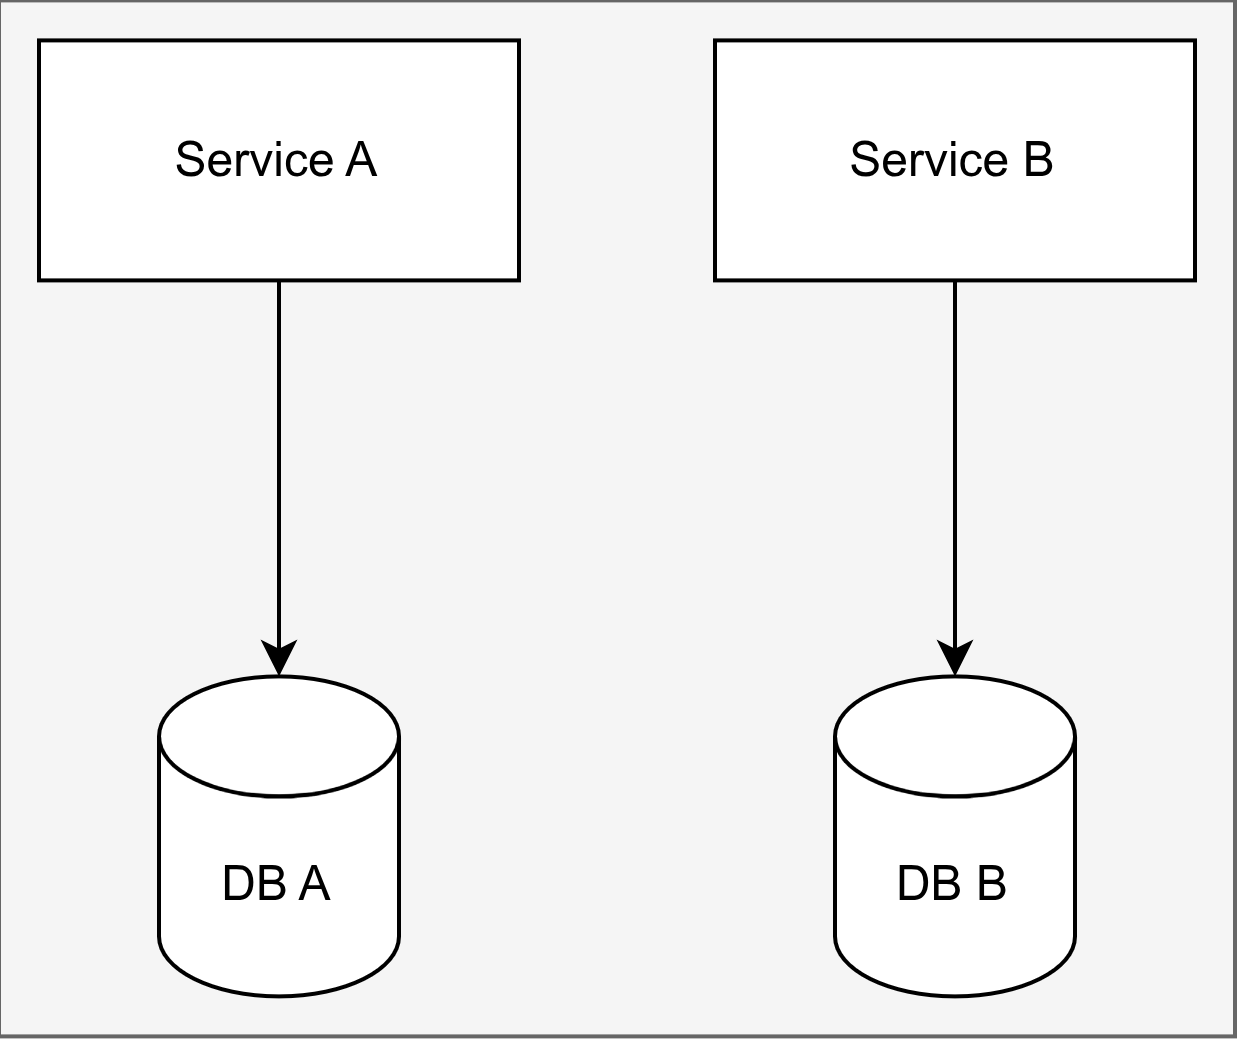
\includegraphics[width=\textwidth,height=0.8\textheight,keepaspectratio]{figures/pattern-01-database-per-service.png}
  \caption{نمط قاعدة بيانات لكل خدمة: تملك كل خدمة قاعدتها، والوصول المتقاطع ممنوع.}
  \label{fig:pattern-01}
\end{figure}

تكمن الغاية من هذا النمط في كسر الارتباط (\en{Coupling}) الذي قد ينشأ نتيجة مشاركة المخططات (\en{Schemas})؛ فحين تشترك خدمتان في قاعدة بيانات واحدة، يصبح أي تعديل في هيكلية الجداول بمثابة تغيير في "عقد ضمني" قد يؤدي إلى تعطل خدمات أخرى دون سابق إنذار. 

بناءً على هذا الأساس، تم تقسيم النظام إلى خمس قواعد بيانات منفصلة: \code{users\_db}، \code{classroomdb}، \code{streaming\_db}، \code{knowledgedb}، و\code{liveassistantdb}. وبالرغم من أن هذا الفصل استلزم استبدال الاستعلامات المباشرة (\en{Joins}) بنداءات بينية بين الخدمات، إلا أنه منحنا مرونة كاملة في تعديل وتوسيع كل خدمة بشكل مستقل.

\subsection{المنافذ والمحوِّلات (\en{Ports and Adapters})}

يهدف هذا النمط (المعروف أيضاً بالمعمارية السداسية) إلى فصل منطق التطبيق عن التفاصيل التقنية للوكلاء الخارجيين. يتم تعريف واجهات مجردة في طبقة التطبيق تسمى "المنافذ"، تصف الاحتياجات الوظيفية، بينما تتولى طبقة البنية التحتية توفير "المحوِّلات" التي تحقق هذه الواجهات. يوضح الشكل~\ref{fig:pattern-02} تطبيق هذا النمط في خدمة المعرفة.

\begin{figure}[htbp]
  \centering
  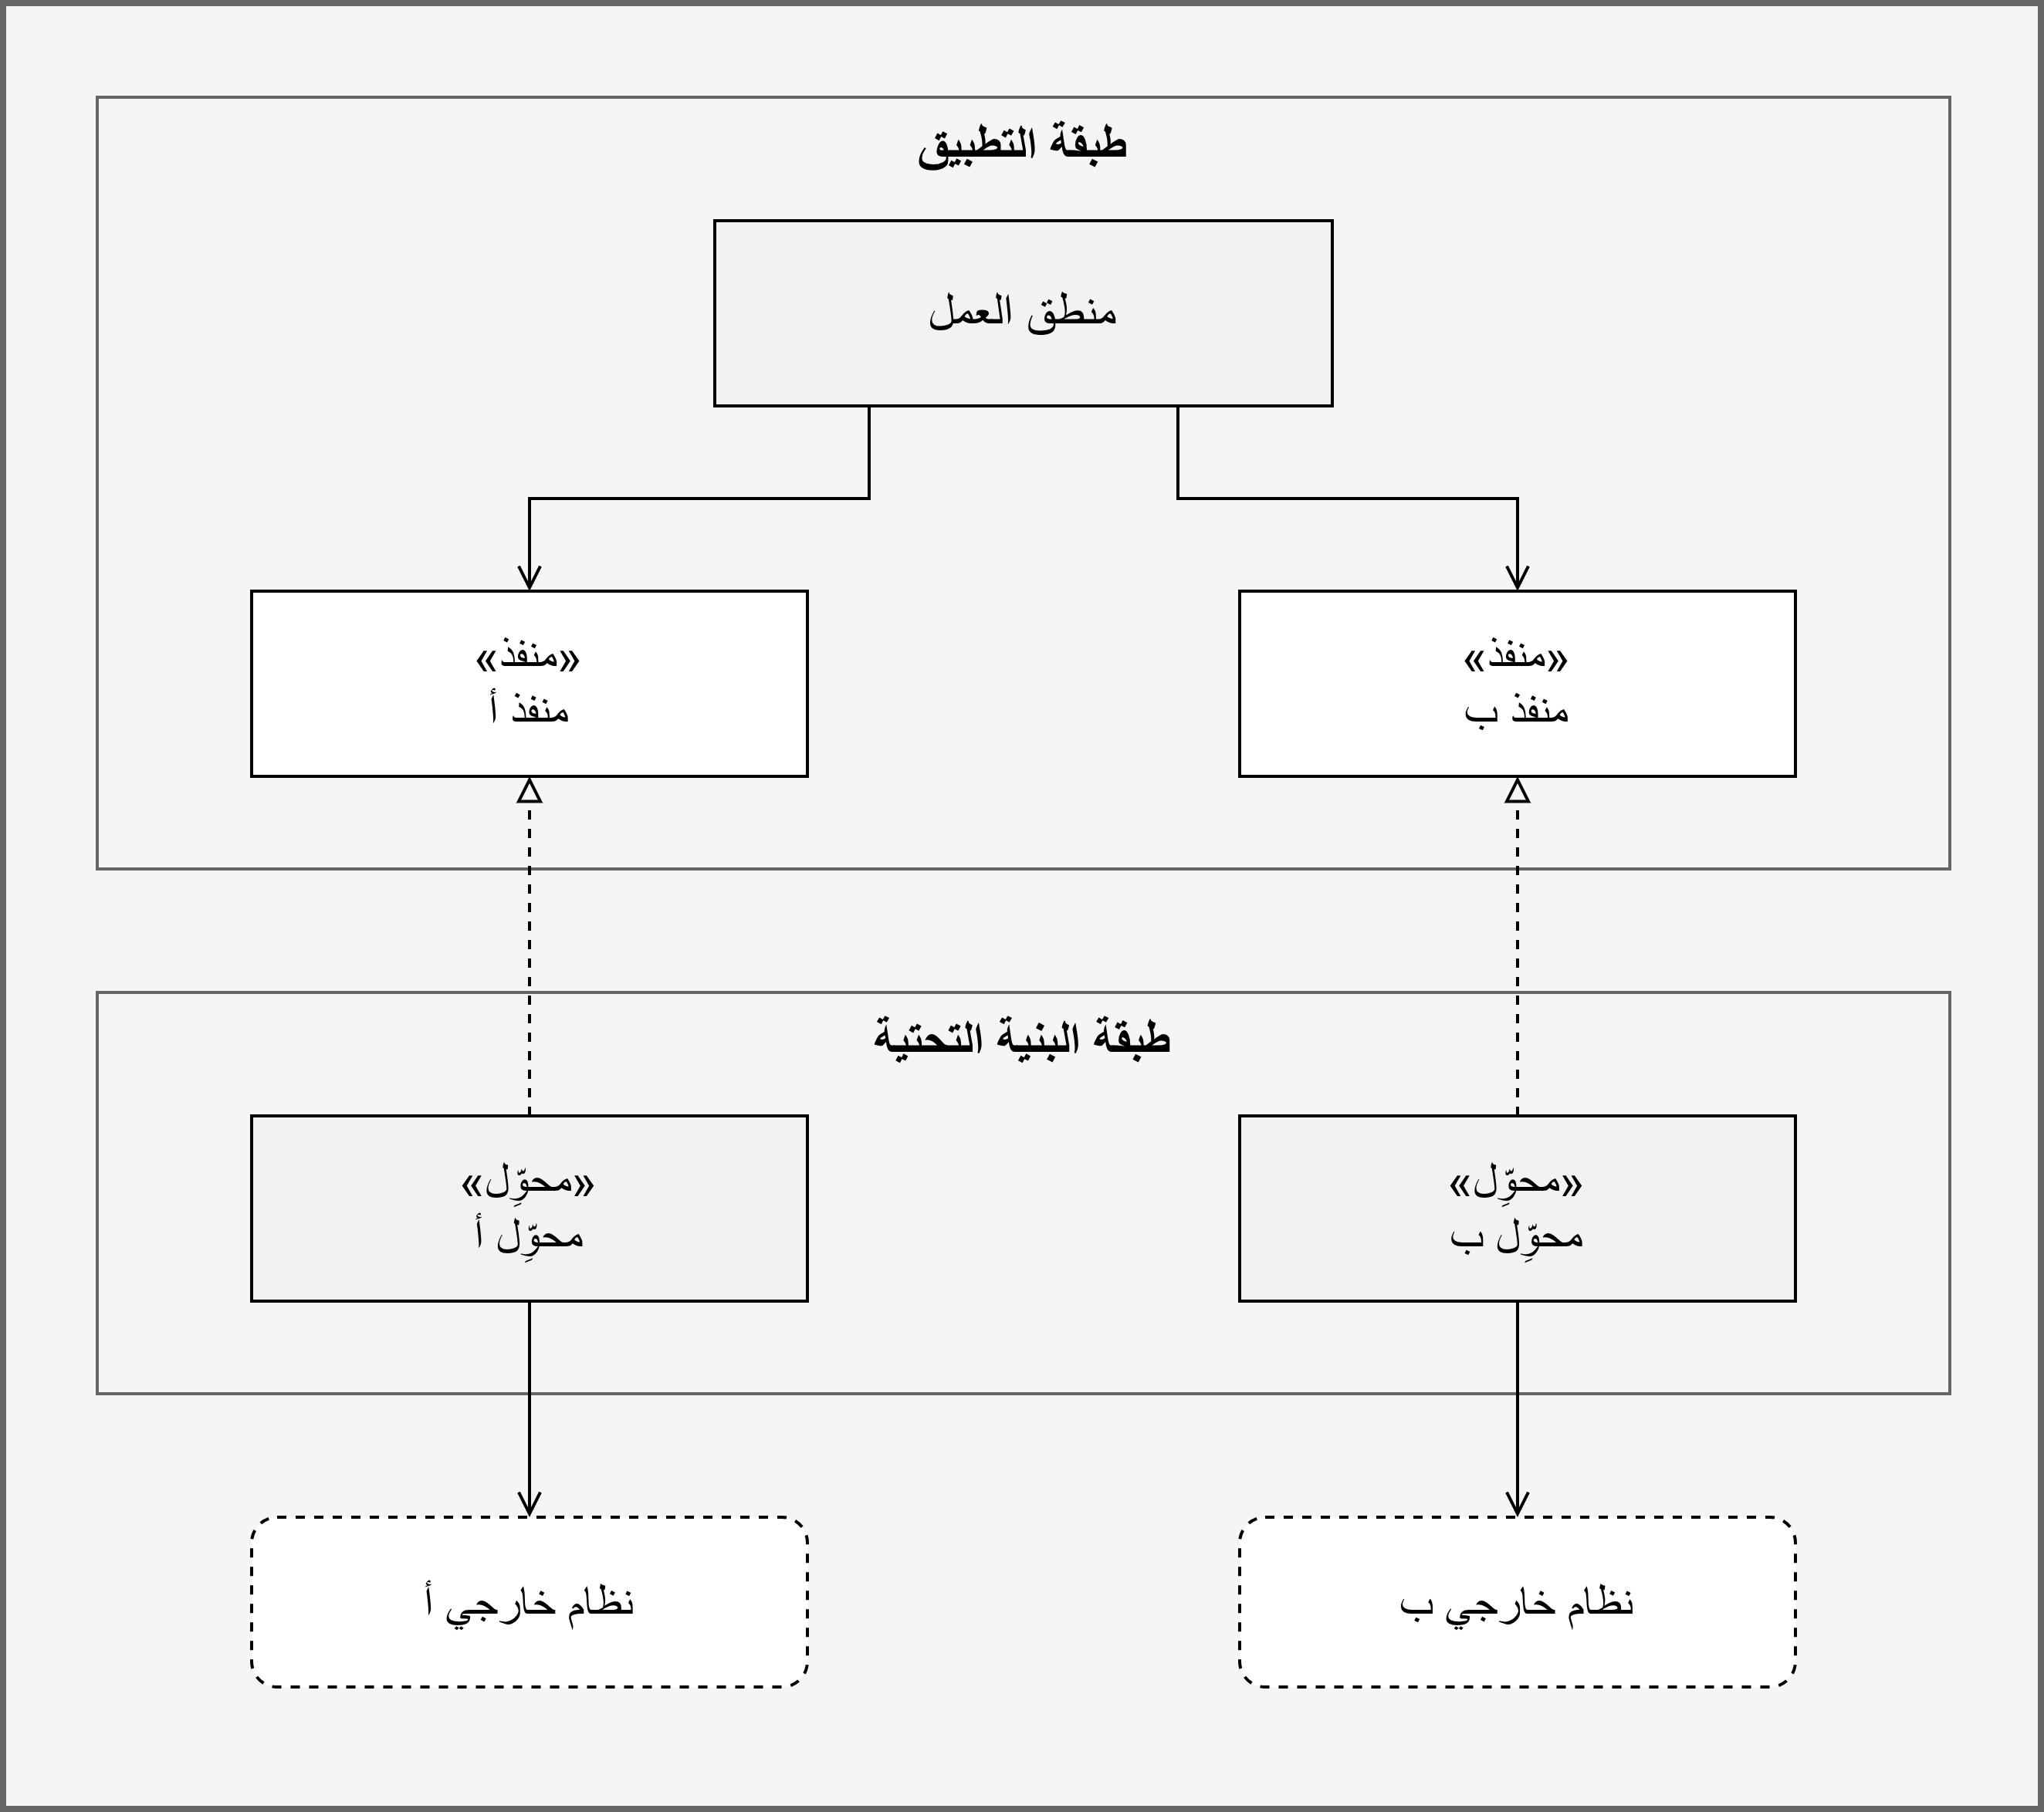
\includegraphics[width=\textwidth,height=0.8\textheight,keepaspectratio]{figures/pattern-02-ports-adapters.png}
  \caption{نمط المنافذ والمحوِّلات: المنفذ يُعرَّف في طبقة التطبيق، والمحوِّل يحقّقه في طبقة البنية التحتية.}
  \label{fig:pattern-02}
\end{figure}

يعالج هذا النمط مشكلة التبعية للتقنيات الخارجية؛ فبدلاً من أن يرتبط منطق العمل بمزود خدمة معين، تصبح الطبقة الداخلية هي التي تملي ما تحتاجه، والخارجية هي التي تلبي ذلك. وقد تم تعريف 14 منفذاً في خدمة المعرفة و8 في خدمة المساعد الحي، مما أتاح لنا اختبار المنطق البرمجي بمعزل عن قواعد البيانات أو خوادم الويب.

\subsection{الاستراتيجية (\en{Strategy})}

يعتمد هذا النمط على تعريف عائلة من الخوارزميات وجعلها قابلة للاستبدال عبر واجهة موحدة، بحيث يمكن للمستدعي استخدام أي منها دون معرفة تفاصيل تنفيذها. يوضح الشكل~\ref{fig:pattern-03} استراتيجيات تحويل الكلام إلى نص (\en{STT}).

\begin{figure}[htbp]
  \centering
  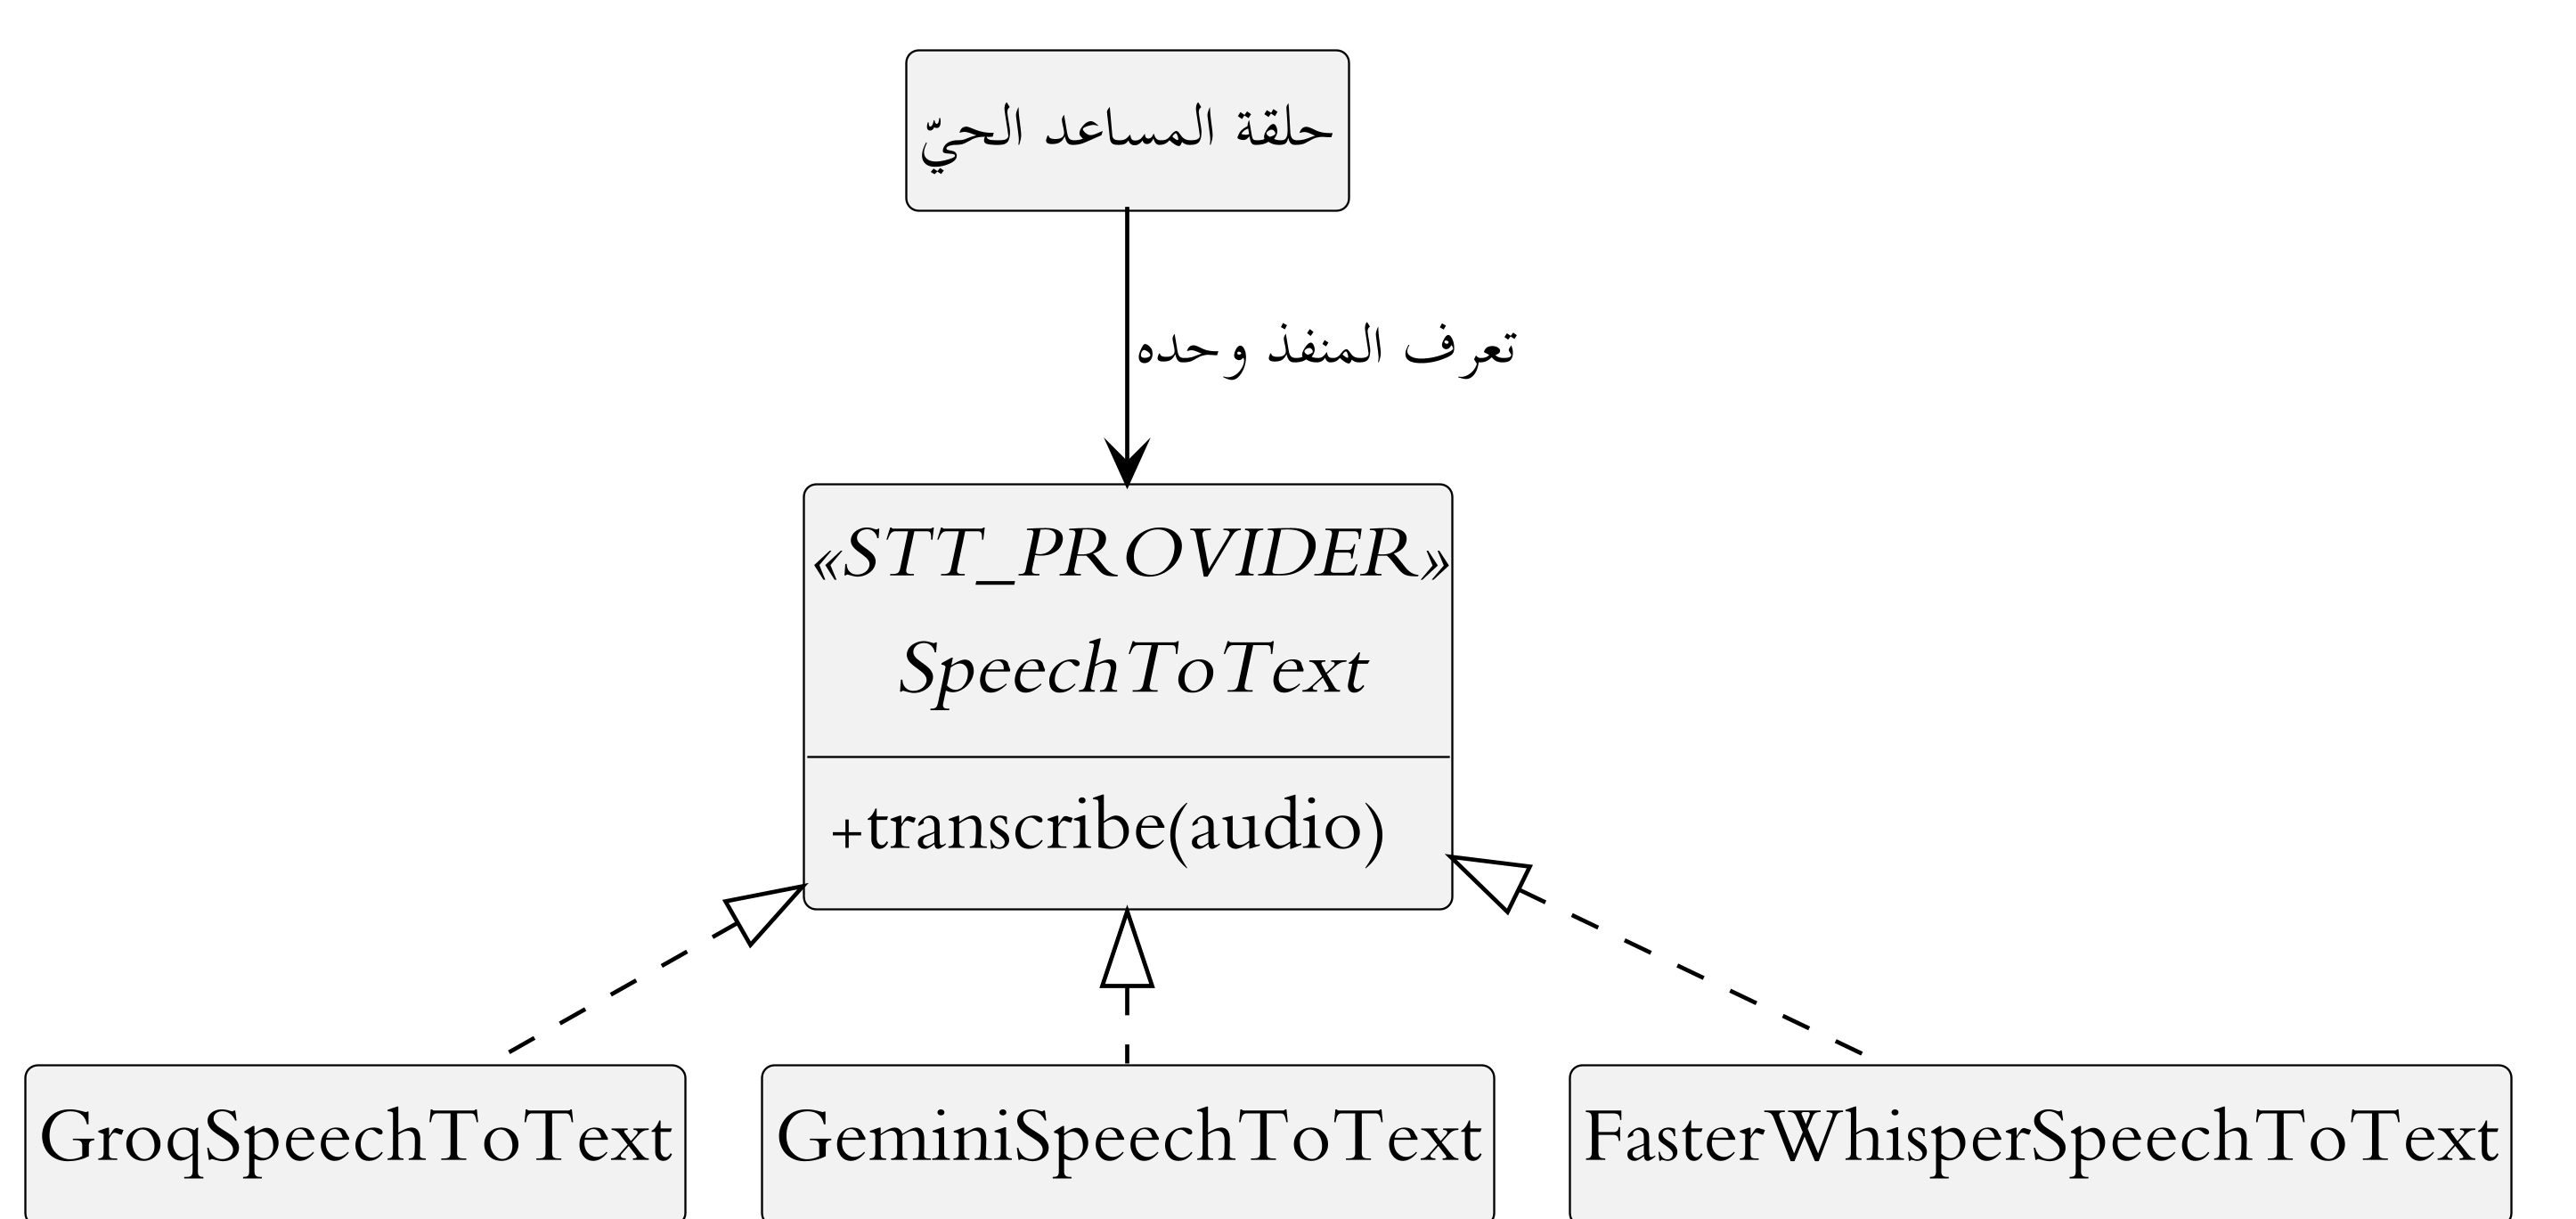
\includegraphics[width=\textwidth,height=0.8\textheight,keepaspectratio]{figures/pattern-03-strategy.png}
  \caption{نمط الاستراتيجية: منفذٌ واحد وثلاثة تحقيقات متكافئة، والمستدعي لا يعرف إلّا المنفذ.}
  \label{fig:pattern-03}
\end{figure}

استُخدم هذا النمط في المواضع التي تتطلب مفاضلة بين بدائل تقنية؛ مثل اختيار نموذج التضمين (\en{Embedding}) أو محرك تحويل الكلام. بفضل هذا النمط، أمكننا الانتقال من النماذج المحلية إلى المستضافة (مثل \en{Gemini}) أو العكس عبر تغيير بسيط في الإعدادات، دون تعديل شيفرة منطق العمل الأساسية.

\subsection{المصنع (\en{Factory})}

يعمل نمط المصنع كمتمم لنمط الاستراتيجية، حيث يتولى مسؤولية اختيار الاستراتيجية المناسبة وإنشائها بناءً على الحالة الراهنة أو الإعدادات، حاجباً بذلك منطق الاختيار عن المستهلك. يعرض الشكل~\ref{fig:pattern-04} مصنع المقسِّمات (\en{Chunkers}) في خدمة المعرفة.

\begin{figure}[htbp]
  \centering
  % Narrower than the rest on purpose: five boxes in four ranks come out taller
  % than wide, and at full width the figure fills the page and floats alone.
  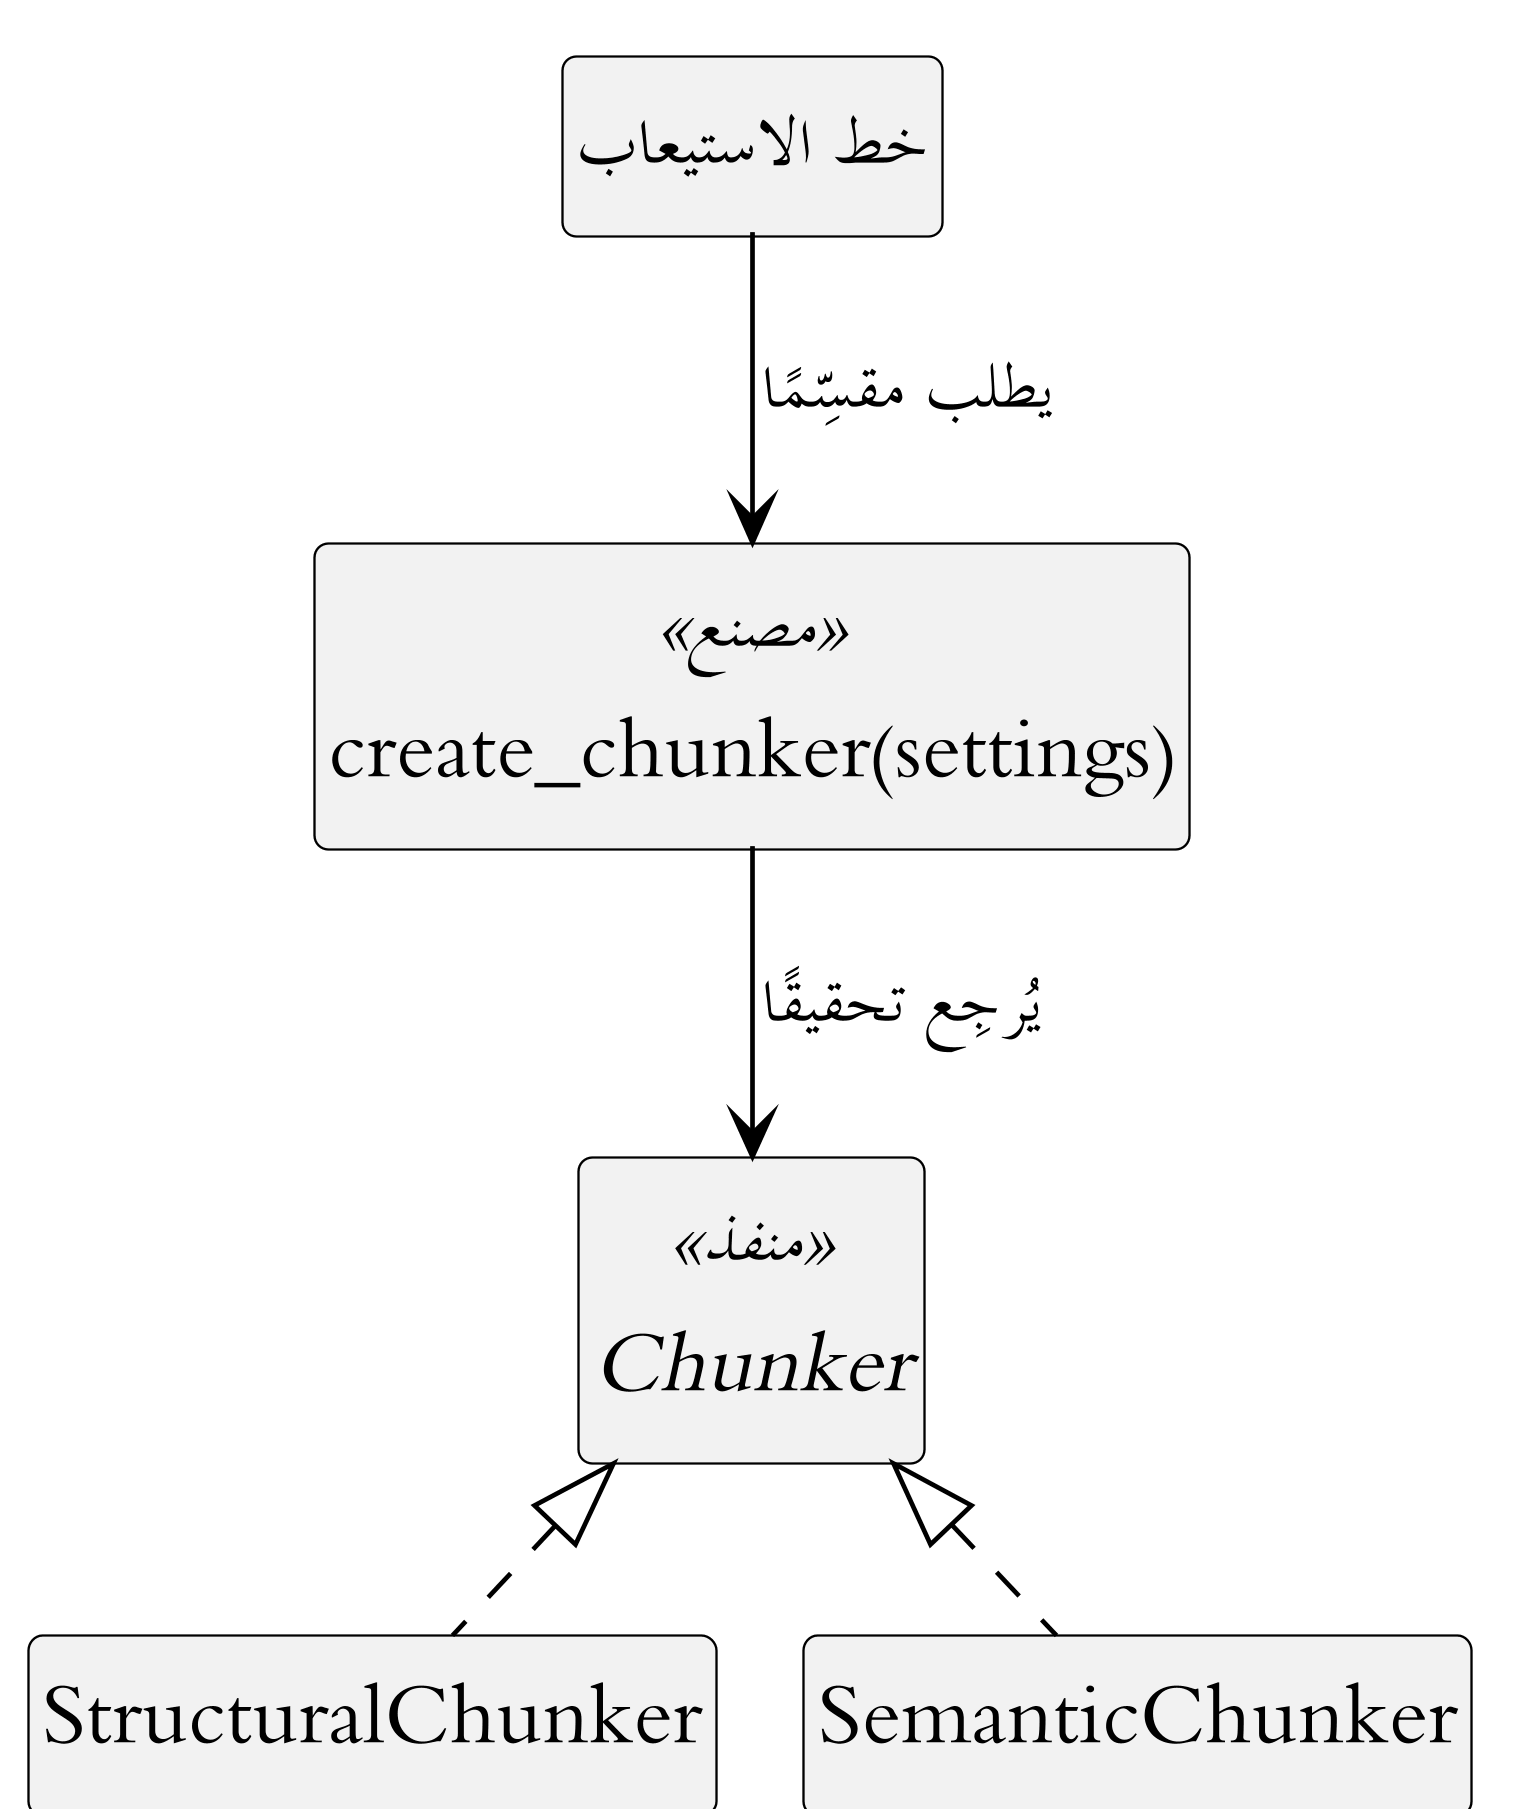
\includegraphics[width=0.6\textwidth,height=0.8\textheight,keepaspectratio]{figures/pattern-04-factory.png}
  \caption{نمط المصنع: المستدعي يطلب مقسِّمًا فيتلقّى تحقيقًا للمنفذ، دون أن يعرف أيَّها.}
  \label{fig:pattern-04}
\end{figure}

في نظامنا، نجد تطبيقات عديدة لهذا النمط، مثل \code{create\_chunker} الذي يقرأ إعدادات التقطيع ويُرجع الاستراتيجية الموافقة، و\code{ExtractorRouter} الذي يحدد المستخرج المناسب حسب نوع الملف المرفوع، مما يضمن بقاء منطق الاستدعاء بسيطاً ومركزاً على المهمة الوظيفية.

\subsection{المستودع (\en{Repository})}

يحجب نمط المستودع آليات الوصول إلى البيانات (مثل استعلامات \en{SQL} أو \en{ORM}) خلف واجهة تتحدث بلغة "المجال التعليمي". يعرض الشكل~\ref{fig:pattern-05} تحقيق هذا النمط في خدمات \en{.NET} عبر قاعدة بيانات عامة.

\begin{figure}[htbp]
  \centering
  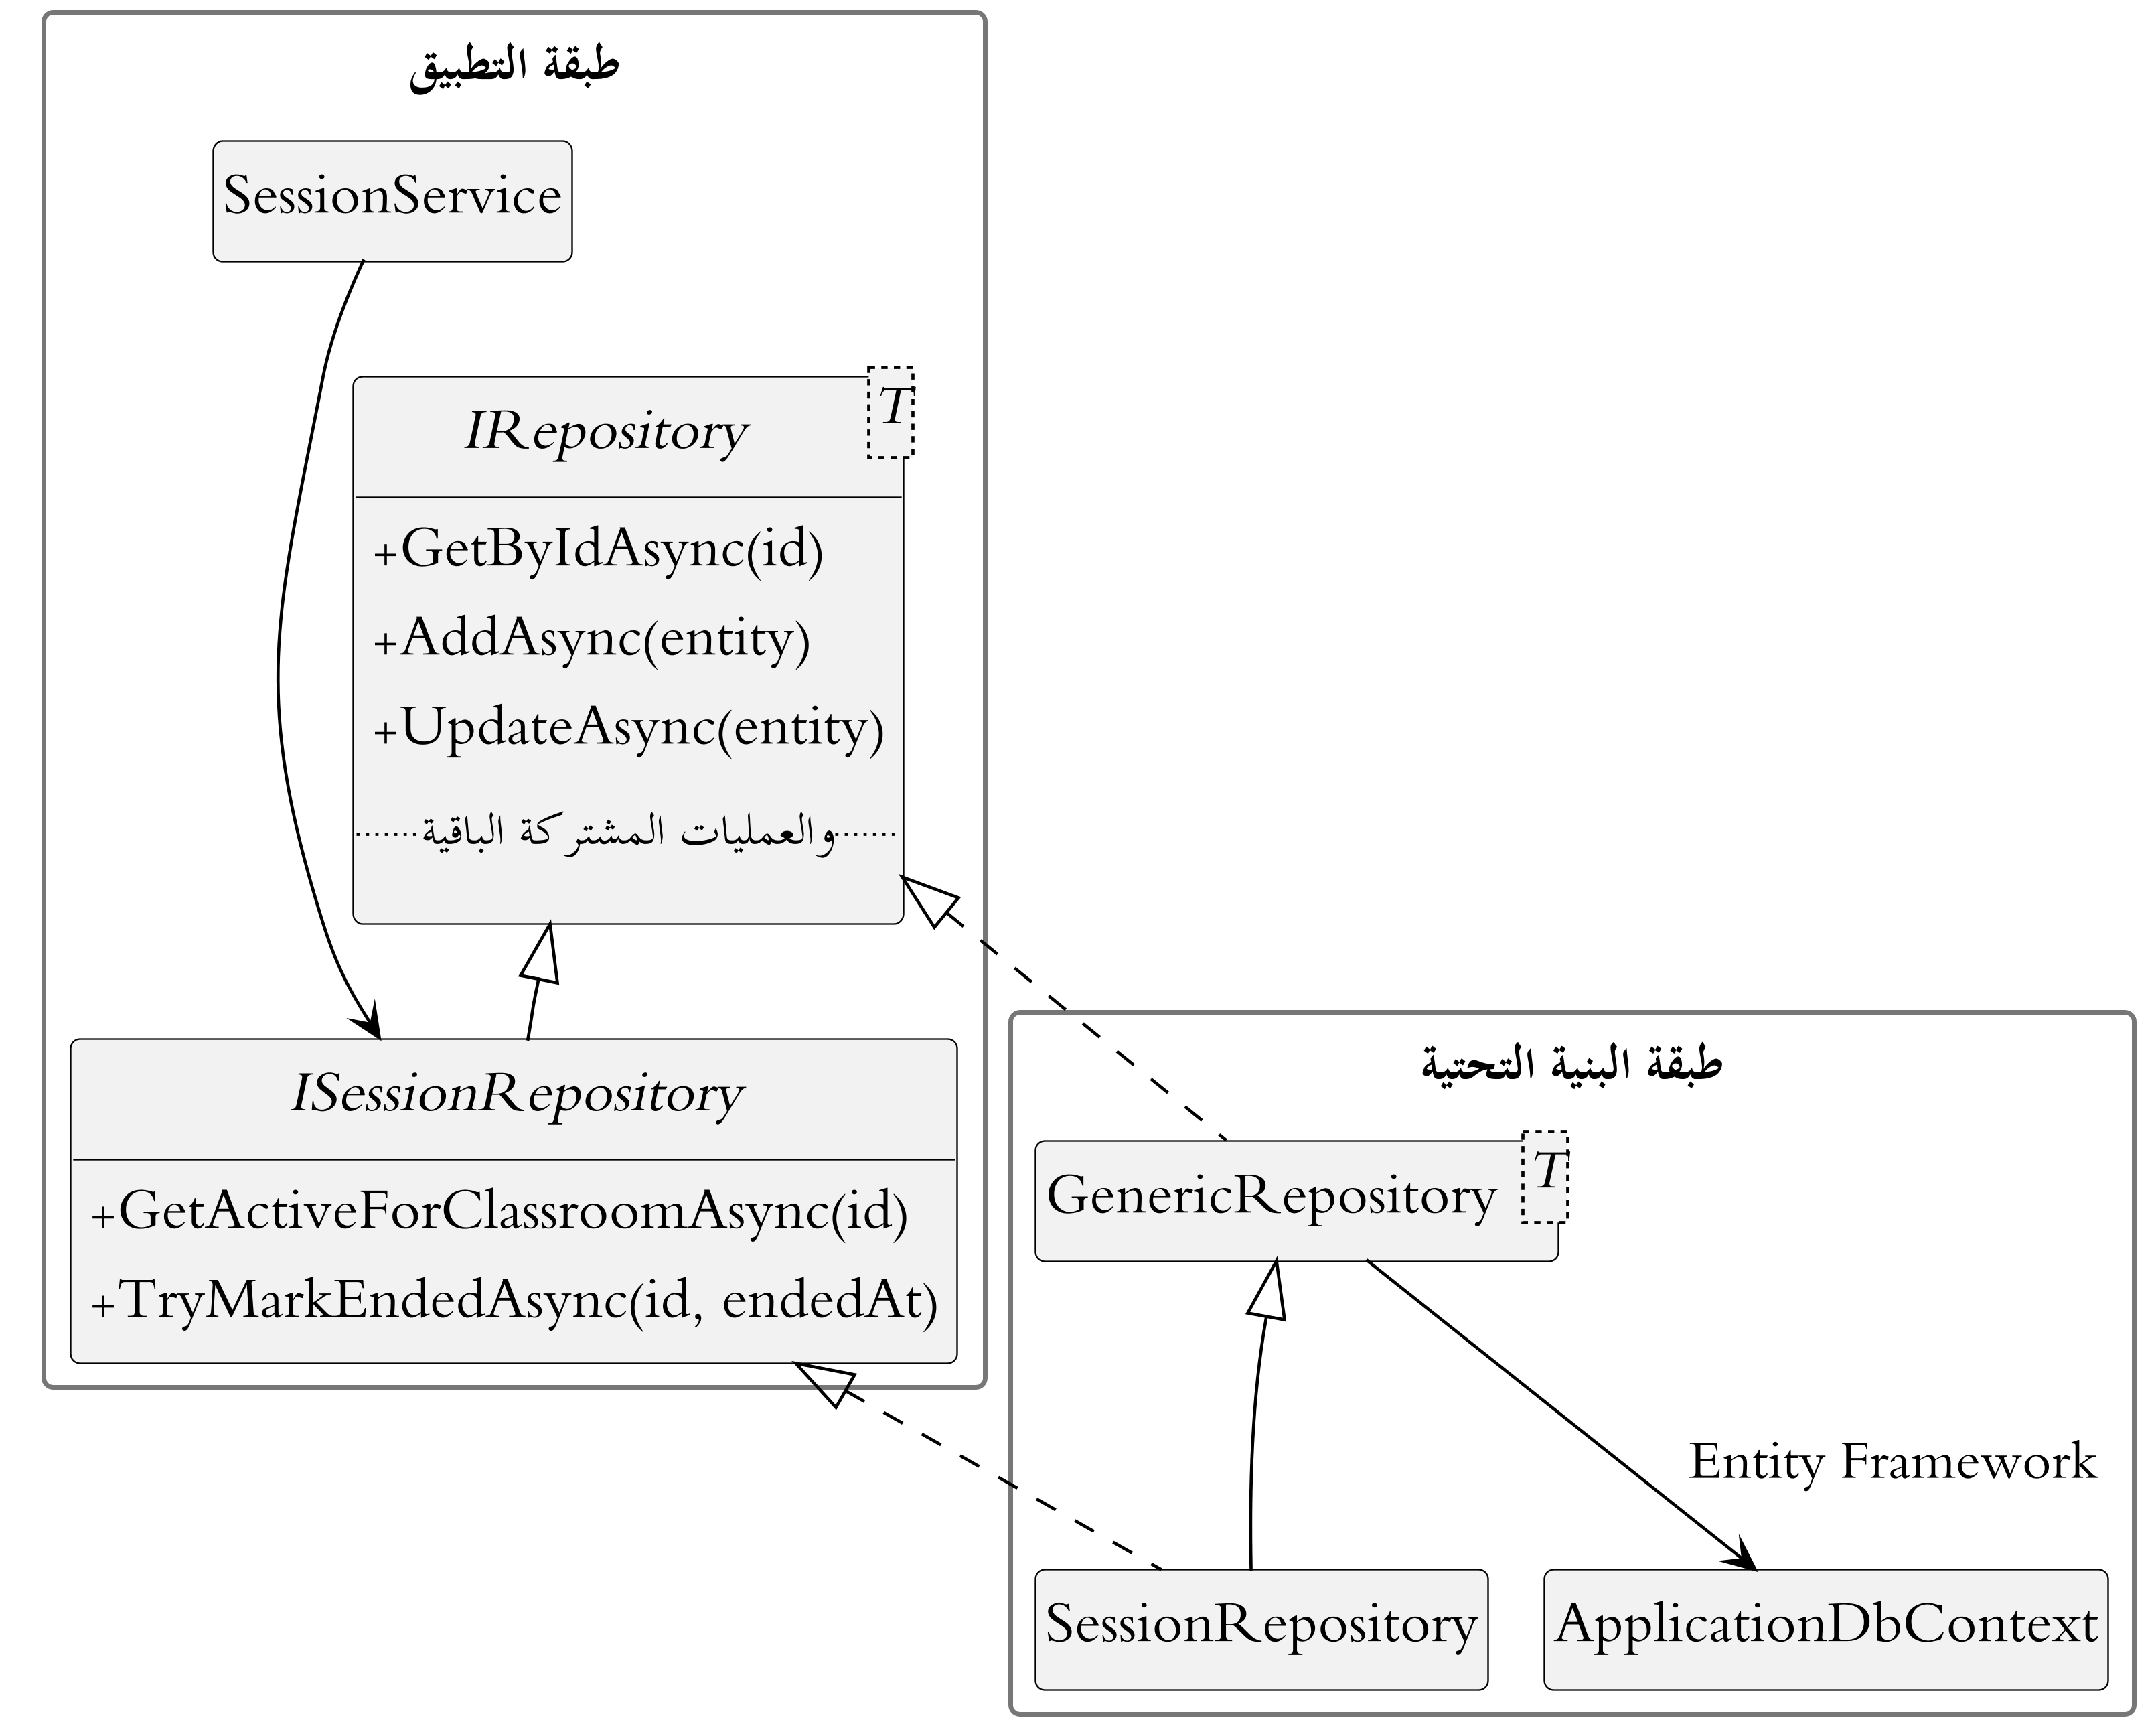
\includegraphics[width=\textwidth,height=0.8\textheight,keepaspectratio]{figures/pattern-05-repository.png}
  \caption{نمط المستودع بقاعدة عامّة: تُعرَّف الواجهة في طبقة التطبيق وتُحقَّق في طبقة البنية التحتية.}
  \label{fig:pattern-05}
\end{figure}

تكمن ميزة هذا النمط في عزل طبقة التطبيق عن مكتبات الوصول إلى البيانات مثل \en{Entity Framework}. وقد اعتمدنا مستودعاً عاماً \code{GenericRepository<T>} يحمل العمليات المتكررة، ورثته عشرة مستودعات متخصصة، مما مكننا من إجراء الاختبارات الوحدوية باستخدام مستودعات وهمية تعمل في الذاكرة دون الحاجة لقاعدة بيانات حقيقية.

\subsection{وحدة العمل (\en{Unit of Work})}

يضمن نمط وحدة العمل جمع عدة عمليات كتابة ضمن معاملة واحدة (\en{Transaction})، بحيث تنجح جميعها معاً أو تُلغى جميعاً، مما يحافظ على اتساق البيانات. يوضح الشكل~\ref{fig:pattern-06} مسار إنهاء الجلسة كمثال على هذا النمط.

\begin{figure}[htbp]
  \centering
  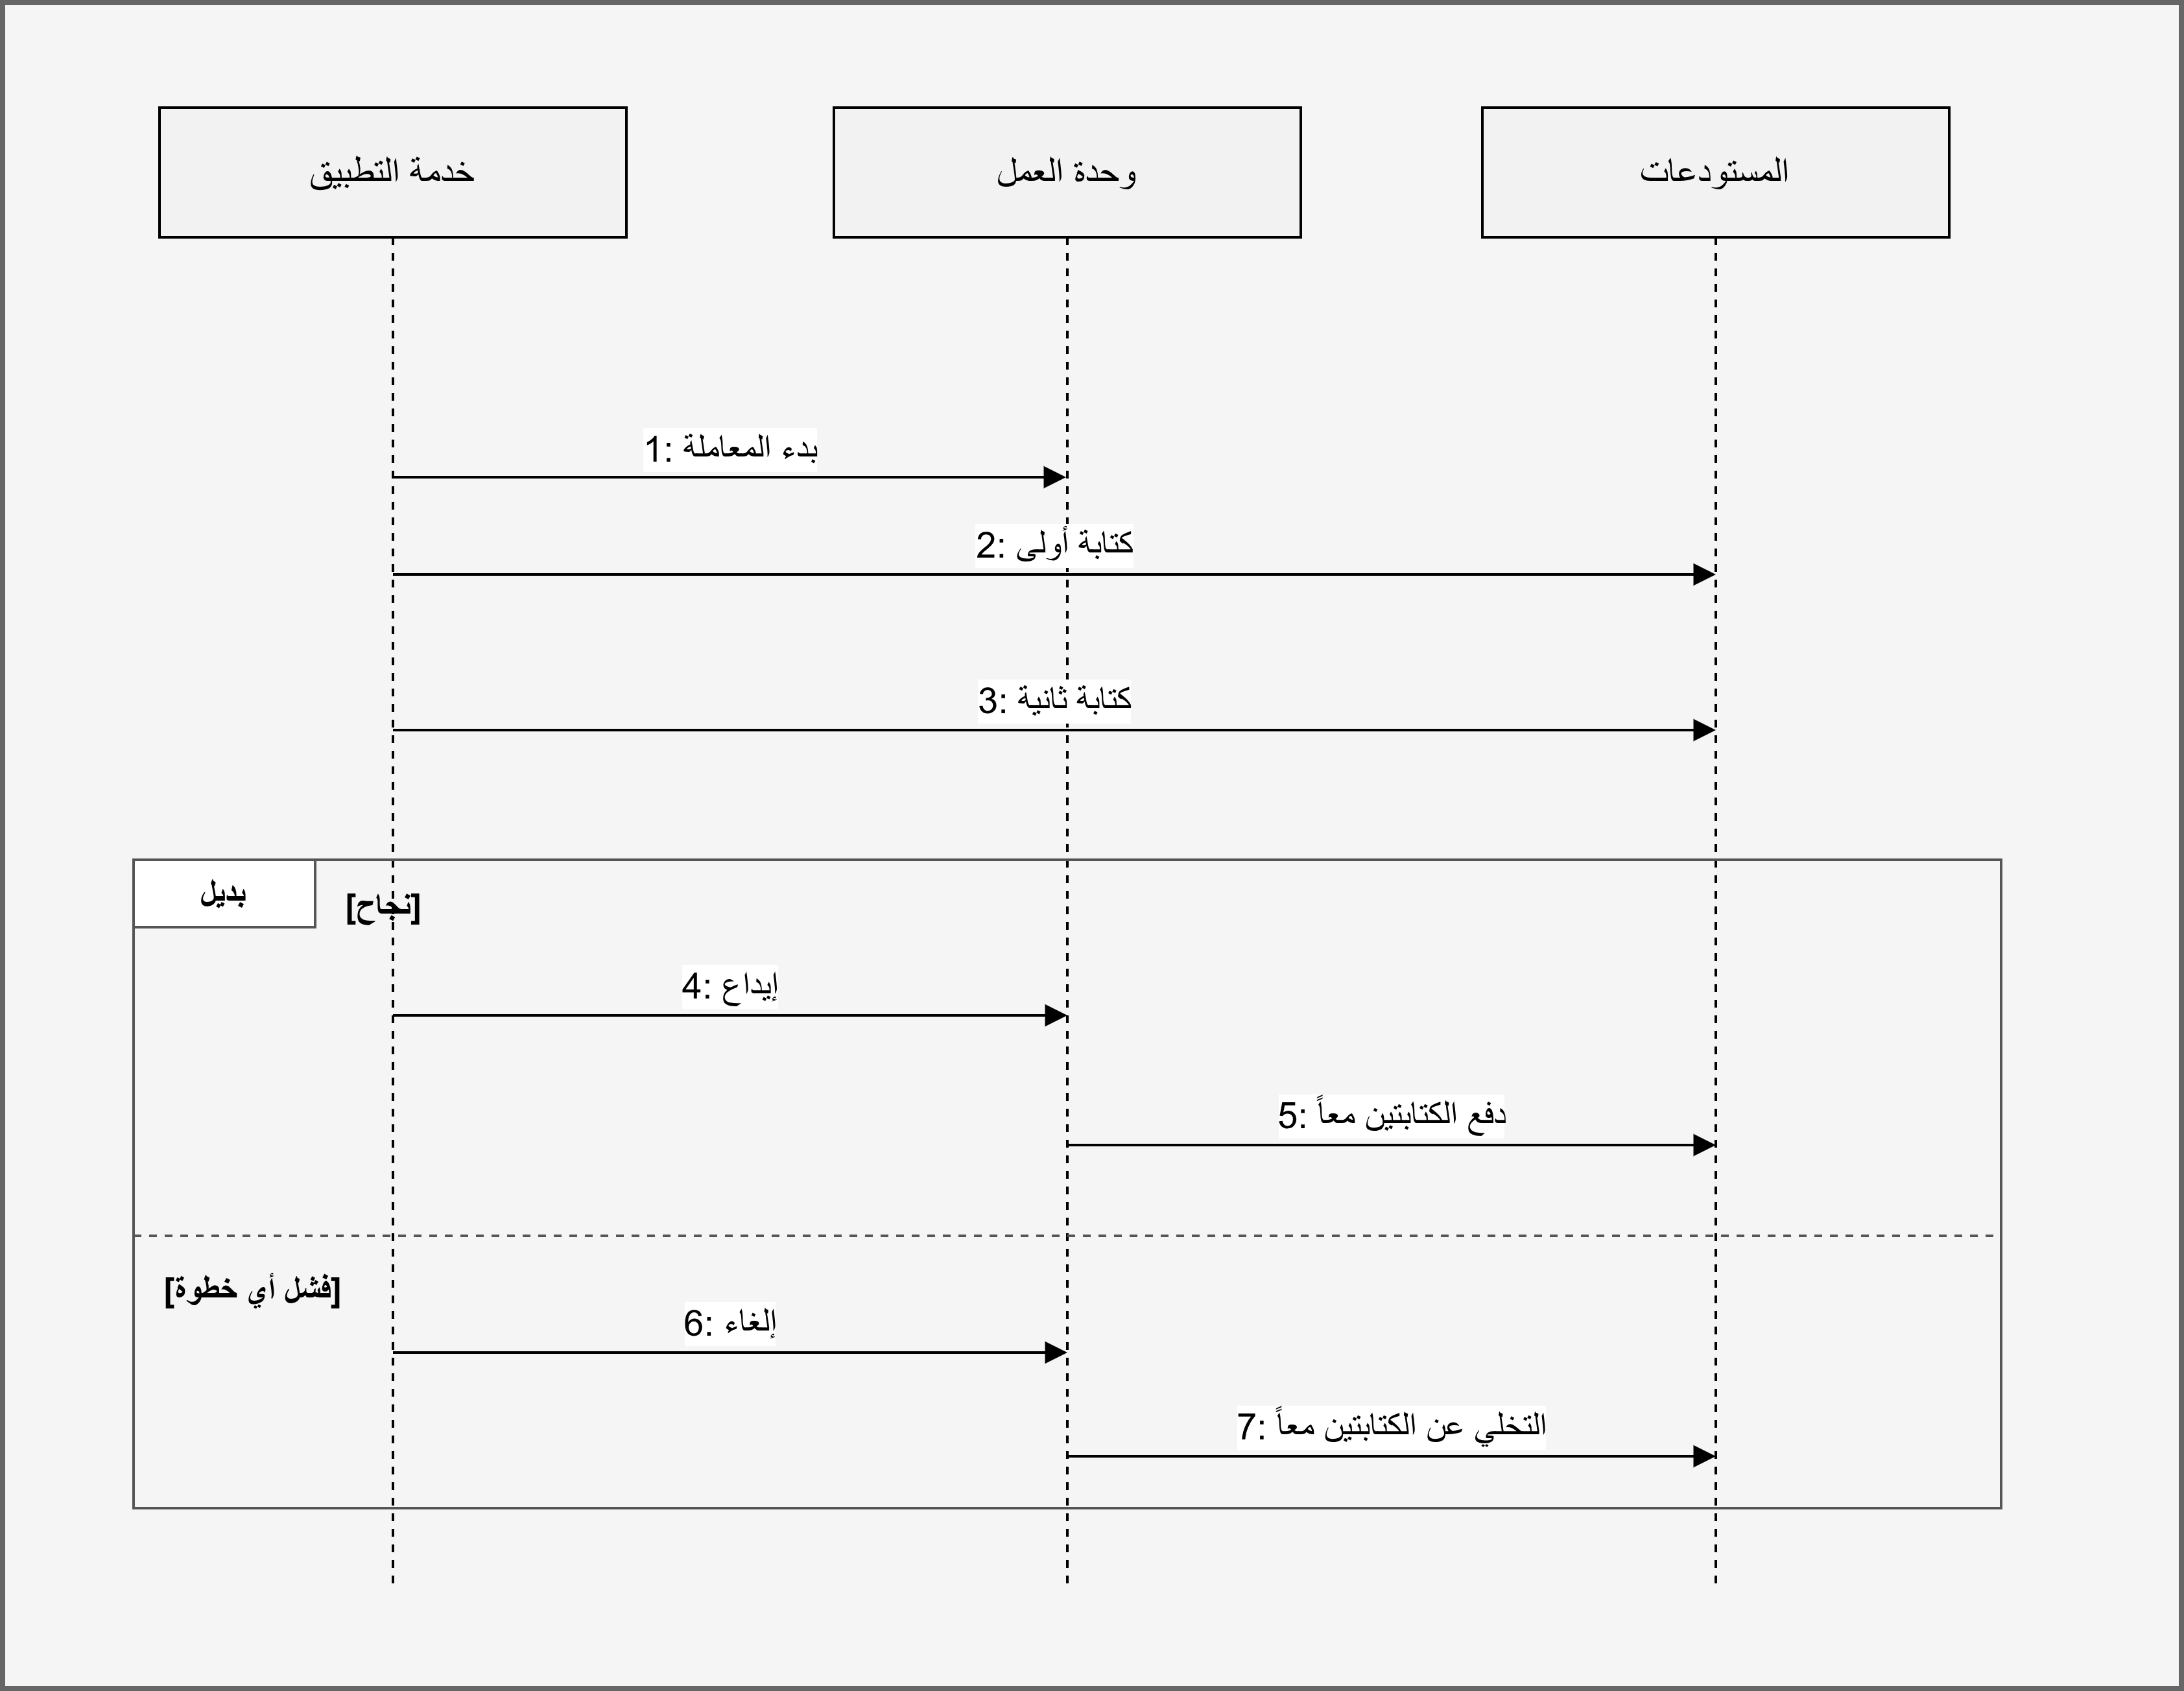
\includegraphics[width=\textwidth,height=0.8\textheight,keepaspectratio]{figures/pattern-06-unit-of-work.png}
  \caption{نمط وحدة العمل: كتابتان عبر مستودعين تحت معاملةٍ واحدة، تُودَعان معًا أو تُلغَيان معًا.}
  \label{fig:pattern-06}
\end{figure}

يعالج هذا النمط مخاطر "البيانات المتناقضة"؛ ففي عملية إنهاء الجلسة، يجب تحديث حالة الجلسة وإضافة سجل الملخص في آن واحد. لولا وحدة العمل، لكان من الممكن تحديث الجلسة وفشل إضافة سجل الملخص، مما يترك النظام في حالة غير متسقة. يوفر المنفذ \code{IUnitOfWork} العمليات اللازمة لإيداع (\en{Commit}) أو إلغاء (\en{Rollback}) المعاملة بشكل آمن.

\subsection{صندوق الصادر المعامل (\en{Transactional Outbox})}

يعد هذا النمط حلاً لمشكلة عدم إمكانية إجراء معاملة ذرية بين قاعدة البيانات وناقل الرسائل (\en{Message Bus}). يعرض الشكل~\ref{fig:pattern-07} آلية عمل هذا النمط لضمان تسليم الأحداث.

\begin{figure}[htbp]
  \centering
  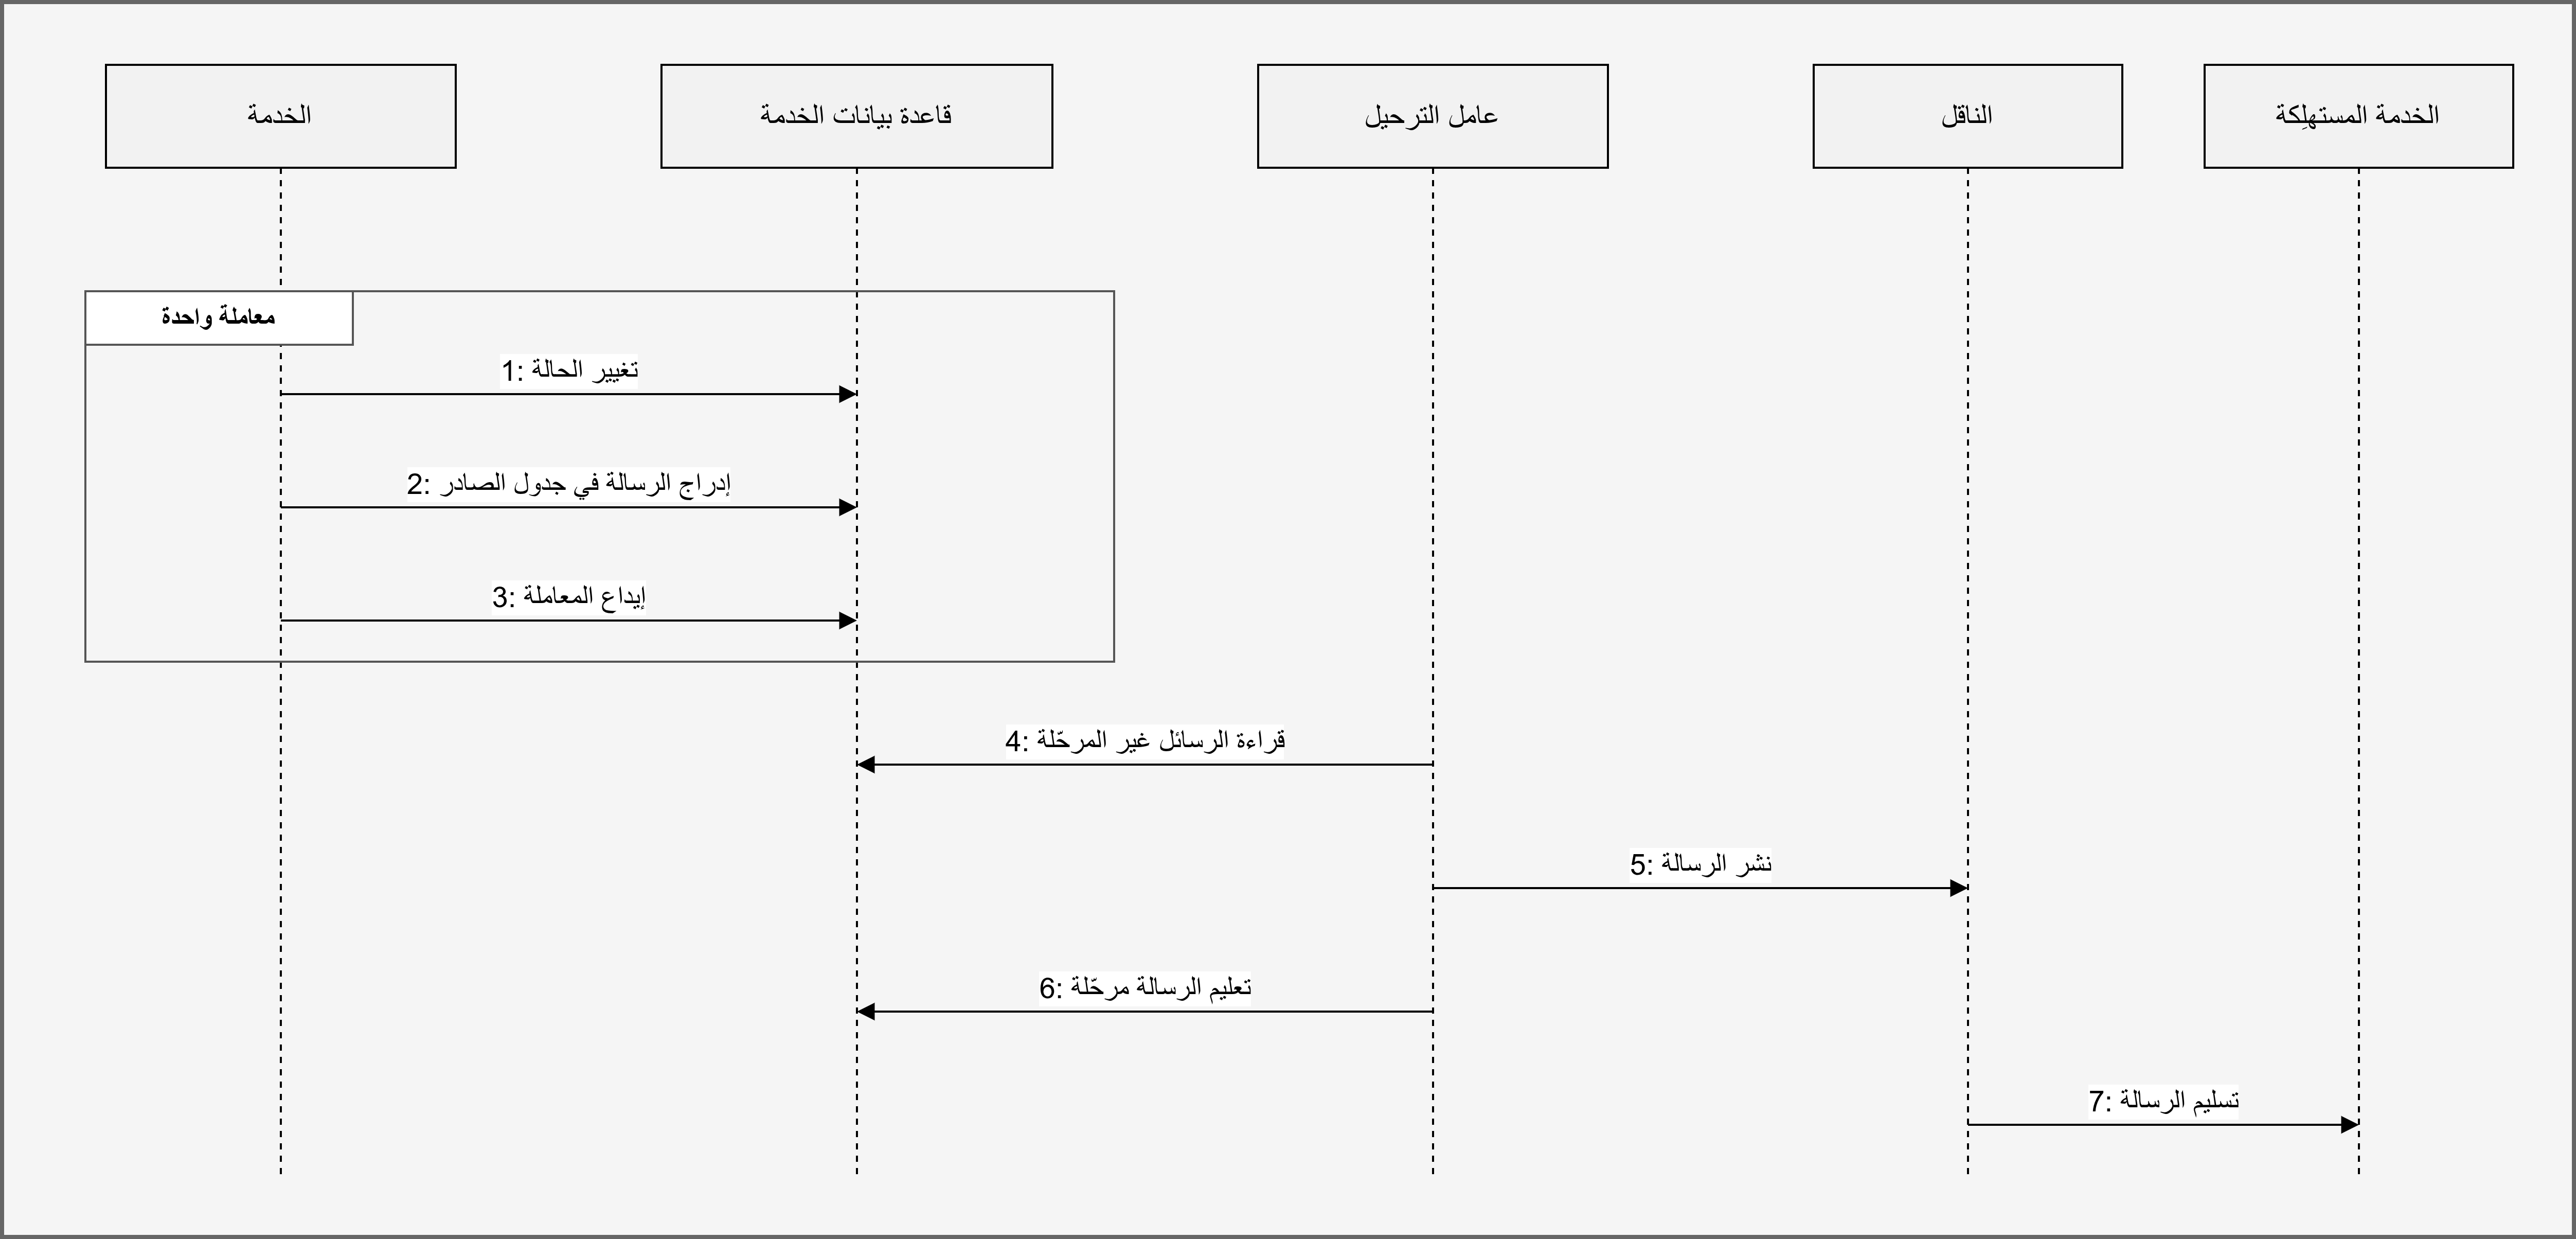
\includegraphics[width=\textwidth,height=0.8\textheight,keepaspectratio]{figures/pattern-07-transactional-outbox.png}
  \caption{نمط صندوق الصادر المعامل: تُكتَب الرسالة ضمن معاملة العمل، ثمّ يُرحّلها عامل مستقلّ.}
  \label{fig:pattern-07}
\end{figure}

عند إنهاء جلسة أو توليد ملخص، تُكتب الرسالة في جدول خاص (\code{outbox\_messages}) ضمن نفس معاملة قاعدة البيانات التي تُغير الحالة. لاحقاً، يتولى عامل ترحيل مستقل قراءة هذه الرسائل ونشرها على الناقل. يضمن هذا الإجراء وصول الإشعارات إلى الخدمات المستهلكة حتى في حال تعطل الناقل لحظياً، حيث تبقى الرسائل في الصادر حتى يتم التأكد من نشرها بنجاح.